\section{Define the Problem of Mapping the Software Applications}\label{sec_problem}
The software applications $A$ are partitioned on the execution platform $\langle N,B\rangle$ by satisfing the user-defined software applications requirements such as applications reliability $\ssp{RL}$, end-to-end timing requirements of chains $\sss{EE}$ and applications criticality $\ssp{cl}$, and by meeting design constrains such as placement restrictions committed by the designer. Essentially, the partitioning is achieved by mapping software-component replicas (or software components) of applications effectively on the computing units $N'$. The partitioning should result in a reduced total power-consumption of the applications $Power(\textbf{x})$, which is achieved by selecting lower-power computing units $N'\subseteq N$, where $\textbf{x}$ is a possible mapping matrix, with \ttxkij representing the mapping of the software component \ttsss{q}[k][i,j] to the compuing unit $n_h$, where $h=\xkij$.  Note: under this partition, the reliability of applications $Reliability_{A_k}(\textbf{x})$, the timing of chains $Delay_{\sss{\Gamma}}(\textbf{x})$ should satify the cooresponding requirements. 

The power consumption of applications as well as the delay of chains depend on the tasks graphs $\bigcup\sss{g}[k][\tau]$, as well as the mapping of the tasks nodes to computing units and the links to the network bus. In this case, the tasks graphs has be constructed from the partition \ttx. However, if the tasks graphs are apriori to the software partitioning problem,  which can be the case if no runnables from different components map to a single task, only the tasks nodes and the links are updated with the mapping information.

\subsection{Task Graph Formulation}
The task graph formulation implies the generation of a task graph \ttat from a runnables graph \ttar in \ttx, and involves two steps: 
\begin{enumerate*}[label=(\roman*)]
	\item updating the mapping information of the runnables according to \ttx, that is for every component type $\sss{c}$ mapped to \ttx, we reterive its runnables $\sss{R}[k][c_i]$. Subsequently, we update the computing units $\sss{\mathcal{N}}[k][r]$ to which the runnables are mapped as show in Equation (\ref{eqn_uprdaterunnables}), in linear-time complexity $O(\sum n_{\ssp{C}}*D)$, where $n_{\ssp{C}}$ are the number of component types in \ttar, $D$ is the maximum degree of replication allowed;
	\item the runnables graph is traversed iteratively to constract the corresponding tasks graph by applying the merging rules as shown in Equation (\ref{eqn_uprdatetasks}), using the method described in Subsection~\ref{subsec_autosarsystem}.
\end{enumerate*}
\begin{align}
\label{eqn_uprdaterunnables}
&\forall ij\forall r\in \sss{R}[k][c_i]\ \sss{\mathcal{N}}[k][r] = n_h \mbox{, where }  h=\xkij &k=1,...,n_A\\
\label{eqn_generatetasksgraphs}
& \ar(\x)\xrightarrow{\text{Eqn. (13);Merging Rules}}\at(\x) &k=1,...,n_A
\end{align}
where \ttgr{\ar} is nodes of the runnables graph \ttar.

However, if the tasks graph is apriori, that is, the runnables-to-tasks is static, only the nodes of the tasks graphs are updated with the mappings information using Equation (\ref{eqn_uprdatetasks}). In the AUTOSAR development, the tasks are usually fixed and the mappings from runnables to tasks is usually static. 
\begin{align}
	\label{eqn_uprdatetasks}
	&\forall ij\forall r\in \sss{T}[k][c_i]\ \sss{\mathcal{N}}[k][\tau] = n_h \mbox{, where }  h=\xkij &k=1,...,n_A
\end{align}

\subsection{Total Power Consumption}
Power consumption refers to the energy usage of electronic components in an integrated circuit, e.g., processor, memory, I/O devices, etc., per time unit. 
There are several models (or techniques) to estimate the power consumption of a computing node. In this work, we use a technique based on processor load (or utilization) to estimate the average power consumption of a computinh node. Specifically, we use the linear polynomial model proposed by Fan et al. \cite{Fan2007PowerComputer}, which is shown in (\ref{eqn_powerconsumption}). The model states that the power consumption of a node is directly proportional to its load, and is inductively formulated from experimental results:
\begin{equation}
\label{eqn_powerconsumption}
\mathcal{P}(u)=P_{idle} + (P_{busy}-P_{idle})*u,
\end{equation}

where $u$ is the utilization of a computing unit, $P_{idle}$ and $P_{busy}$, respectively refer to the power consumption measured at minimum and maximum processor loads. The measurements can be obtained by running performance benchmark suits, e.g., MiBench \cite{Guthaus2001MiBench:Suite}, AutoBench \cite{EMBC2018AutoBenchProcessors}, etc. The utilization of the computing units for a partition $\textbf{x}$ is computed as a sum of the utilization of their respective constituent tasks as shown in Equation (\ref{eqn_util_node}). Finally, the total power-consumption of the applications is the sum of the power-consumption of the units as shown in Equation (\ref{eqn_total_power}).
\begin{align}
\label{eqn_util_task}
\mathcal{U}(\tau)              & =  \frac{\mathrm{WCET}_\tau}{P_\tau}\\
\label{eqn_util_node}
(u_1,...,u_{n_N})&=\sum_{k=1}^{n_A}\sum_{\tau\in V(\at)(\x)}{(\mathcal{U}(\tau)|Node_\tau=n_h, h=1,..,n_{N})}\\
\label{eqn_total_power}
\mathcal{P}_{total}(\textbf{x})  &=\sum_{h=1}^{n_N}{u_h(\x)}  
\end{align}
where $\mathcal{U}$, in Equation (\ref{eqn_util_task}), computes utlization of task $\tau$ as a ration of its worst-case execution time and period, and $u_h$ is utilization of node $n_h$.

%The applications requirements are modeled as constraints that need to be satisfied in the allocation problem. The constraints formulations are shown in the following subsections, respectively for reliability, timing and other design constraints such as related to runnables-to-tasks merging and replication.

\subsection{Software-Applications Reliability Constraints}\label{subsec_reliability_constraint}
The applications reliability constraints ensure the mapping $\textbf{x}$ satisfies the user-defined reliability requirements, that is $\forall k\ \rel_{A_k}(\x)\leq RelReq_{A_k}$. 
The reliability of each application is computed over $t$ period of time from the computing units \ttssp{N} and  the shared network bus $B$, where \ttssp{N} hosts \ttar. The reliability is computed assuming exponentially distributed and constant failure rates of the units $\lambda_{n_h}$ as well as the network bus $\lambda_B$. Thus, the reliability of an application is computed as a product of the reliability of the units and the network bus as shown using Equation (\ref{eqn_appreliability_app}). Note: if application does not use the shared  bus $\rel_{B}=1$. Equation (\ref{eqn_nodes_app}) finds the units \ttssp{N} that the application \ttar uses by traversing the partition \ttx in linear time.
\begin{align}
	\label{eqn_appreliability_app}
	&Reliability_{\ar}(\x)=Reliability_{\ssp{N}}(\x)*Reliability_B\\
	\label{eqn_nodes_app}
	&\ssp{N}=\{e\in N| \forall ij\ e=m_h\},\mbox{ where } h=\ssx{k}{ij}
\end{align}
Note: we assume applications are mutuallye exclusive, that is no shared components exist between any two applications, therefore, we can safety calculate the reliability of applications independently. Consequently, to increase readability, we remove the superscript $(A_k)$ in the rest of this subsection.

The reliability of the units is $Reliability_N(\x)=e^{-\lambda_N(\x) t}$, where is $\lambda_N(\x)$ is the failure rate of an $N$-unit system over the partition \ttx. The system failure-rate is computed using the state enumeration as shown in \cite{Lucet1999ExactReliability}, which is an exact technique to calculate reliability, as opposed to using series-parallel technique - motivated in Subsection \ref{sub_reliability}. By applying the state enumeration technique, the system failure-rate can be defined as the probability a software application \textit{fails} in the probability space $\langle \Omega,\xi,p,f\rangle$.
\begin{itemize}
	\item $\Omega=\{0,1\}$ are the possible outcomes (or states) of a computing unit. Assume the Boolean variable $s_h\rightarrow\Omega$, which indicates the state of $n_h$, then $s_h=0$ indicates $n_h$ fails and $s_h=0$ indicates $n_h$ operates. Thus, for computing units $N=\{n_1,..,n_{n_N}\}$, the states of the units (or configuration) is indicated by the $N$-cardinality set $S=\{s_1,...,s_{n_N}\}$.
	
	\item $\xi=\Omega^S$ are elementary events that correspond to the possible configurations of the units $N$, therefore, the events are mutually exclusive. Consider $N=\{n_1,n_2,n_3\}$, Table (\ref{tbl_application_rel}) shows the their possible configurations $\xi$. Assume the configuration $s\in \xi=\{0,1,0\}$, it shows $n_1$ and $n_3$ fail as indicated by $s_1=0,s_3=0$, respectively, and $n_2$ operates as indicated by $s_2=1$. 
	
	\item $p:\xi\rightarrow[0,1]$ assings the configurations probabilities using
	\[\forall s\in \xi\  p_s=\prod_{h=1}^{n_N}{\lambda_{n_h}*(1-s_h)+(1-\lambda_{n_h})*s_h}\]
	where $\lambda_{n_h}$ is the failure-rate of $n_h$. The probability $p_s$ is the product of the probability of having the state $s_h$, which is $\lambda_{n_h}$ if $n_h$ fails, otherwise, $(1-\lambda_{n_h})$ if $n_h$ operates.
	
	\item $f:\xi\rightarrow \{0,1\}$ determines the status of the applciation in each state $s\in\xi$, that is $f_s=0$ means the application fails, otherwise, $f_s=1$ means the application operates, at the sate $s$.
\end{itemize}

\begin{table}
	\centering
	\begin{tabular}{@{}llll@{}}
		\toprule
		Units Config. & Probability & Comonent Status & Application Status \\ 
		$s\in\xi$   & $p_s$     & $\forall i\ s_{c_i}$ & $f_s$ \\ \midrule
		$\{0,0,0\}$ & 0.0000000000 & $\{0, 0, 0\}$        & 0     \\
		$\{0,0,1\}$ & 0.0000000099 & $\{0, 0, 1\}$         & 0     \\
		$\{0,1,0\}$ & 0.0000000099 & $\{1, 0, 0\}$          & 0     \\
		$\{0,1,1\}$  & 0.0000999800 & $\{1, 1, 1\}$         & 1     \\
		$\{1,0,0\}$ & 0.0000000099 &$\{1, 0, 1\}$         & 0    \\
		$\{1,0,1\}$ & 0.0000999800 & $\{1, 1, 1\}$        & 1     \\
		$\{1,1,0\}$ & 0.0000999800 & $\{1, 1, 1\}$          & 1     \\
		$\{1,1,1\}$ & 0.9997000299 & $\{1, 1, 1\}$           & 1     \\ \bottomrule
	\end{tabular}
	\caption{Example of Application Reliability Calculation using State Enumeration Over 10-years Operational Lifetime: an Application with Component Types $C=\{c_1,c_2,c_3\}$, Replicas $Q=\{c_{1,1},c_{1,2};c_{2,1},c_{2,2};c_{3,1},c_{3,2}\}$ Partitioned on $N=\{n_1,n_2,n_3\}$ according to Figure (\ref{fig_deployment}), the Variable $s_{c_i}\in\{0,1\}$ Indicates if the Replicas of Type $c_i$ Fails or Functions, Respectively.}
	\label{tbl_application_rel}
\end{table}

%The fact that an application functions $f_s$ is defined via its inverse, which is \textit{software application failure}, deductively as follows:
\begin{definition}[Software Application Failure]
A software application fails in the configuration $s\in\xi$ if there exists a component type $c_i$ where all of its replicas $Q_i$ \textit{fail}, otherwise, it functions, as shown using Equation (\ref{eqn_app_failure}).  The component replica $q_i,j\in Q_i$ of type $c_i$ fails if $n_h$ fails, that is $s_h=0$.
\begin{align}
\label{eqn_app_failure}
f_s(\x)&= 
\begin{cases}
0 & \mbox{ if } \exists i\ c_i|\forall j\ s_h=0\\
1 & \mbox{ otherwise }
\end{cases}&\mbox{ where }h=x_{ij}
\end{align}
\end{definition}

Thus, the failure rate of the $N$-unit system $\lambda_N(\x)$ is the sum of the probabilities in which the application fails, that is
\[
	\lambda_N(\x)=\sum_{s\in \xi|f_s(\x)=0}p_s(\x)
\]
\begin{example}[Reliability Calculation]
Let us assume we want to calculate the reliability of the application in Table~\ref{tbl_application_rel} over a 10-year (or 87600h) operational lifetime. The reliability of the units is $\rel_N=e^{-\lambda_N t}=0.99736671$, where $\lambda_N=p_1+p_2+p_3+p_5=0.0000000301$. Assume $\lambda_B=0.00000001$, hence $\rel_B=e^{-\lambda_B t}=0.99912438$. Then, the reliability of the application is $\rel_N*\rel_B=0.99649339932$.
\end{example}



\subsection{Chains Timing Constraints}
The chains timing constraints over \ttx ensure that the delays of chains meet thier respective end-to-end requirements, that is $\forall k\forall \gamma\in \ssp{\Gamma}\ Delay_\gamma(\x)\leq \sss{\mathrm{EE}}[k][\gamma]$. The delays calculations require that the tasks and messages in the chains meet their deadlines. Since, each task is used in at least one chain, we check the schedulability of all tasks and the message  before we calculate the chains timing constraints. The schedulability of the tasks and the message is checked using the worst-case response-time anlaysis presented in Subsection \ref{subsec_responsetimeanalysis} and  Subsection \ref{subsec_responsetimeanalysis}, respectively. Moreover, the schedulability of the chains is checked using the age-delay analysis shown in Subsection \ref{subsec_causeeffectchains}. 

\subsubsection{Tasks Timing Constraints}
The tasks timing constraints ensure that the tasks in the distributed system meet their respective deadlines. Tasks replicas mapped to the same unit do not improve realiability of the applications since we assume a permanent failure of computing units would lead to the total failure of the software running on the units. Consequently, the replicas except one are discarded, hence exists only a maximum of one replica per computing unit. The replica can be identified from other replicas based on the unit to which it is mapped. Assume $\tau\in \gr{V}{\at}$ is a task node and $\sss{\mathcal{N}}[k][\tau]$ is the set of units to which its replicas can be mapped. Thus, the replicas of $\tau$ are represented a paired-set $\mathcal{R}=\{(\tau,n)|n\in\sss{\mathcal{N}}[k][\tau]\}$, where $(\tau,n)$ is the replica of $\tau$ mapped to $n$.
\begin{figure}[h!]
	\centering
	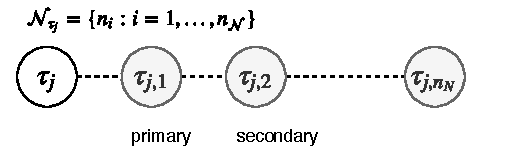
\includegraphics[width=0.7\linewidth]{img/task_replicas}
\end{figure}

To constract the tasks timing constraints, first we arrange the tasks per computing unit, $\ssb{T}[n_h]$, so that the tasks graphs are not traversed everytime the response-time of tasks is computed. So, we traverse the tasks graphs, consequently in each task node $\tau\in V(\at(\x))$, we check if the replica $\tau_{i,j}$ is mapped to $n_h\in N$. If the condition is true, we collect the task node $\tau_i$ as shown in Equation (\ref{eqn_tasks_nodes}). 
\begin{align}
\label{eqn_tasks_nodes}
T_{n_h}&=\{\tau\in \mathcal{V}(\at(\x)) | \forall j\in\sss{\mathcal{N}}[k][\tau_i][b]\ j=n_h\} & \mbox{ for all } h=1,...,n_N,
\end{align}
where $\mbox{ where }h=\xkij$. The complexity of this equation, considering an adjucency matrix implementation, is exponential time $O(\sum{|\gr{V}{\at}|*n_N^2})$, where $\gr{V}{\at}$ is tasks nodes in $\at$, and $N$ is the total computing units in the distributed system. 

Subsequently, we calculate the response time of each task $\tau \in T_{m}$ in \ttx by invoking the response-time analyais formula, and construct the tasks timing constraints as shown in Equation (\ref{eqn_tasks_constraints}).
\begin{align}
\label{eqn_tasks_constraints}
\forall \tau\in T_{n} \ ResponseTime_\tau(\x)&\leq Deadline_\tau
\end{align}

\subsubsection{Messages Timing Constraints}
The messages timing constraints ensure that the response-time of message in the CAN bus meet their respective deadlines, which is equal to their periods. The messages $M$ in \ttx are determined from the communication links of the tasks graphs. Assume $(t1,t2)\in\gr{E}{\at}$ is a link in the task graph. Due to replication, the link represents a set of sub-links $\sss{\mathcal{R}}[k][t2][b]\times\sss{\mathcal{R}}[k][t2][b]$ that communicate the replicas of $t1$, $\sss{\mathcal{R}}[k][t1][b]$, and the replicas of $t2$, $\sss{\mathcal{R}}[k][t2][b]$. Thus, if the task $(t1,n1)\in\sss{\mathcal{R}}[k][t1][b]$ and $(t2,n2)\in\sss{\mathcal{R}}[k][t2][b]$ are mapped to the same  computing units, that is $n1=n2$, the link is not mapped on the bus, rather uses a shared variable or inter-process communication. Whereas, if the tasks are mapped on different units, the link is mapped to a bus, hence a message is used to establish the communication between the tasks. Equation (\ref{eqn_tasks_nodes}) shows how the messages in the distribured systems are determined by traversing the sub-links of the tasks graphs, 
\begin{equation}
\label{eqn_tasks_nodes}
M=\{m_i | \forall (t1,t2)\in \mathcal{E}(\atx)\forall (i,j)\in\sss{\mathcal{R}}[k][t1][b]\times\sss{\mathcal{R}}[k][t2][b]\ n_i\neq n_j\},
\end{equation}
where $(i,j)$ is a sub-link of $(t1,t2)$, $m_{i}$ is the message that the replica $i$ uses to communicate with the replica $j$.  We assume the message arrival behavior is periodic, similar to $t1$, i.e., $P_{m_i }= P_{t1}$. Likewise, it herits its criticality from $t1$, i.e., $\mathrm{CL}_{m_i}=\mathrm{CL}_{t1}$, so that the criticality is preserved at the network, as well.

\subsubsection{Delay  Constraints}
The delay calculation of chains is multiplicity due to replication. Assume the chain $\Gamma=(\tau_i)_{i=1}^l=(\tau_1,...,\tau_l)$, then the set of chains with replication is a cartesian product of the tasks replicas (or the tasks nodes mapping to computing units according to $\x$) in the chain, that is $\Gamma^*(\x)= \sss{\mathcal{R}}[k][\tau_1][b]\times,...,\times\sss{\mathcal{R}}[k][\tau_l][b]$, where $l$ is the chain length. Assume we want to calculate the delay of the chain $\gamma\in \Gamma^*$ compositionally, where $\gamma=(t_i)_{i=1}^l=(t_1,...,t_l)$: first we identify the subchains $I$ and messages $J$ of the chain. The subchains $I$ are subsets of the chain $\gamma$ where the communication between the sender and receiver tasks of the chain use a network bus. That is, if $t_i$ is the sender task, and its receiver task $t_{i+1}$ is mapped to a different unit, i.e., $n_{t_i}\neq n_{t_{i+1}}$, then $(t_h)_{h=i'}^i\in I$ is a subchain of $\gamma$ and $m_{t_i}\in J$ is the message used by the subchain, where $0\leq i'\leq i$, captured by the expression
$
	(I;J)=\{(t_i)_{i=0}^{l-1};m_{t_i} | n_{t_i}\neq n_{t_{i+1}}\}
$.
	
Thus, the delay $\Delta_\gamma(\x)$ for a mapping \ttx is computed as the sum of the age delays of its subchains and the response-times of the messages,
\[
	\Delta_{\gamma}(\x)=\sum_{i\in I_{\gamma}(\x)}{\Delta^{sub}_{i}(\x)} + \sum_{j\in J_{\gamma}(\x)}{\delta^{msg}_i(\x)},
\]
according to the age-delay formula shown in Equation (\ref{eqn_agedelay_multinode}), where $\Delta^{sub}$, $\delta^{msg}$ are the functions that compute the age delay of $i$ subchain, and the response-time of $j$ message, respectively. Thus, the chains timing constraints are formulated over \ttx and applications $A$ using Equation (\ref{eqn_chains_constraints}).
\begin{align}
\label{eqn_chains_constraints}
\forall \gamma \in \ssp{\Gamma} \ \sss{\Delta}[k][{\gamma}](\x) & \leq \sss{\mathrm{EE}}[k][\gamma],
\end{align}
\begin{example}[Delay Calculation] Consider the chain $\Gamma=\tau_1\rightarrow\tau_2\rightarrow\tau_4$ from Figure~\ref{fig_appexample} where $\tau_1$ and $\tau_2$ realize the component types $c_1$, and $\tau_4$ realizes $c_2$. The mapping of the components is shown in Figure~\ref{fig_deployment} (b), i.e., with replication. Thus, the units to which $\tau_1$ and $\tau_2$ are mapped are $\sss{\mathcal{R}}[k][\tau_l][b]=\sss{\mathcal{R}}[k][\tau_2][b]=\{n_1,n_2\}$, and $\tau_4$ to $\sss{\mathcal{R}}[k][\tau_4][b]=\{n_2,n_3\}$, by infering the mappings of respective components. Table~\ref{tbl_chains_with_replication} illustrates how compute the chains, considering replication of degree 2, which is $\Gamma^* = \sss{\mathcal{R}}[k][\tau_1][b] \times \sss{\mathcal{R}}[k][\tau_2][b] \times \sss{\mathcal{R}}[k][\tau_4][b]$, and also how to compute the subchains and messages of each chain $\gamma\in \Gamma^*$. The delays of the subchains is computed according to the age-delay semantics demonstrated in Subsection~\ref{subsec_cause_effect_chains}.
\end{example} 
\begin{table}[]
	\begin{tabular}{@{}lll@{}}
		\toprule
		$\gamma\in \Gamma^*$ & $i\in I_\gamma$ & $j\in J_\gamma$ \\ \midrule
		$(\tau_1,n_1)\rightarrow (\tau_2,n_1)\rightarrow(\tau_4,n_2)$ & $(\tau_1,n_1)\rightarrow (\tau_2,n_1),(\tau_4,n_2)$ & $m_{(\tau_2,n_1), (\tau_4,n_2)}$ \\
		$(\tau_1,n_1)\rightarrow (\tau_2,n_1)\rightarrow(\tau_4,n_3)$ & $(\tau_1,n_1)\rightarrow (\tau_2,n_1),(\tau_4,n_3)$ & $m_{(\tau_2,n_1), (\tau_4,n_3)}$ \\
		$(\tau_1,n_2)\rightarrow(\tau_2,n_2)\rightarrow(\tau_4,n_2)$ & $(\tau_1,n_2)\rightarrow(\tau_2,n_2)\rightarrow(\tau_4,n_2)$ & $\emptyset$ \\
		$(\tau_1,n_2)\rightarrow(\tau_2,n_2)\rightarrow(\tau_4,n_3)$ & $(\tau_1,n_2)\rightarrow(\tau_2,n_2),(\tau_4,n_3)$ & $m_{(\tau_2,n_2), (\tau_4,n_3)}$ \\ \bottomrule
	\end{tabular}
\caption{Chains-with-Replication of Degree 2 for the Chain $\Gamma=\tau_1\rightarrow\tau_2\rightarrow\tau_4$, its Subchains $I$ and Messages $J$.}
\label{tbl_chains_with_replication}
\end{table}

\subsection{Approximation of Delay Calculation}
Due to the replication, the number of chains-with-replication per chain $\Gamma$ grows exponentially as the degree of the replication $D$ linearly increases, $|\Gamma|^D$. Likewise, the length of the chain has a polynomial effect as it grows. Moreover, the age-delay calculation is exhaustive search as demonstrated in the example. For these main reasons, the delays computation is normall expesive. Such computationally expensive operations are challenging for metaheuristics, due meta-heuristic algorithms compute large-space candidate solutions. Therefore, we propose an appoximation algorithm to efficiently compute the delays by selecting only the chain-with-repications that use the buses the most.






\subsection{Software Allocation Optimization	}\label{sec_allocation}
The software allocation is defined as a single-objective optimization problem. The objective function  $Power(\x)$ is a cost function which minimizes the total power consumption of the software applications as deployed in the heterogenuous computing units, where \ttx is the decision variable (or solution) of the optimization. The cost function is formulated in Equation \ref{eqn_optimization}, with inequality constraints shown by Equation (\ref{eqn_reliability}, \ref{eqn_responsetime},\ref{eqn_e2e}). The constraints ensure the solution meet the reliability requirements, the tasks deadlines,  and the chains end-to-end requirements.  Furthermore, the overlapping constrain shown in Equation (\ref{eqn_overlapping}) ensure that replicas are not allocated to the same computing units.
\begin{align}
\label{eqn_optimization}
\min_{\textbf{x}\in X}\ Power(\textbf{x}) & &\text{ subjected to:} \\
\label{eqn_reliability}
\rel_{A_k}(\x)&\leq RelReq_{A_k} & \mbox{ forall } k=1,...,n_{A_k}\\
\label{eqn_responsetime}
\forall \tau\in T_{m_h}\    ResponseTime_{\tau}(\x)&\leq Deadline_{\tau}& \mbox{forall } h=1,...,n_{M}\\ 
\label{eqn_e2e}
\forall \gamma \in \ssp{\Gamma}\  Delay_\gamma(\x)&\leq E2eReq_\gamma& \mbox{forall } k=1,...,n_{A}\\
%\label{eqn_overlapping}
%\forall k\forall ij\ x_{ij}^{(k)}&\neq x_{ij}^{(k')},&  \mbox{ where } k\neq k'=1,...,n_{rep}
\end{align}
where $X$ is the search space of the problem, $\textbf{x}\in X$ is a feasible solution, and $\xkij\in \textbf{x}$ is a mapping of a component $\sss{q}[k][i,j]$ to the node $m_h$, where $h=\xkij$
%
%In the rest of this section, we show the ILP model and the PSO algorithm of the software allocation problem, which are validated on an automotive use case and evaluated for performance in the next section. Throughout this section, we use a simple running example of a system model in order to demonstrate our proposed ILP model and the PSO optimization algorithm.
%
%\subsection{Running Example}
%The example employs an AUTOSAR system, which consists of a software application model and a hardware platform model, as well as functional and extra-functional requirements such as timing and reliability of the software application. The software application is modeled as a digraph of runnables, which is shown in Figure \ref{fig_application}. It consist of 50 runnables, 35 cause-effect chains (or paths), with their activation patterns and timing specifications shown in Table \ref{tbl_requirements}. The timing specifications of the runnables as well as the software components from which the runnables are instantiated are shown in Table \ref{tbl_comps_config}. The hardware platform model consists of three computation nodes, with specifications shown in Table \ref{tbl_nodes_specification}.
%\begin{figure}[t!]
%\centering
%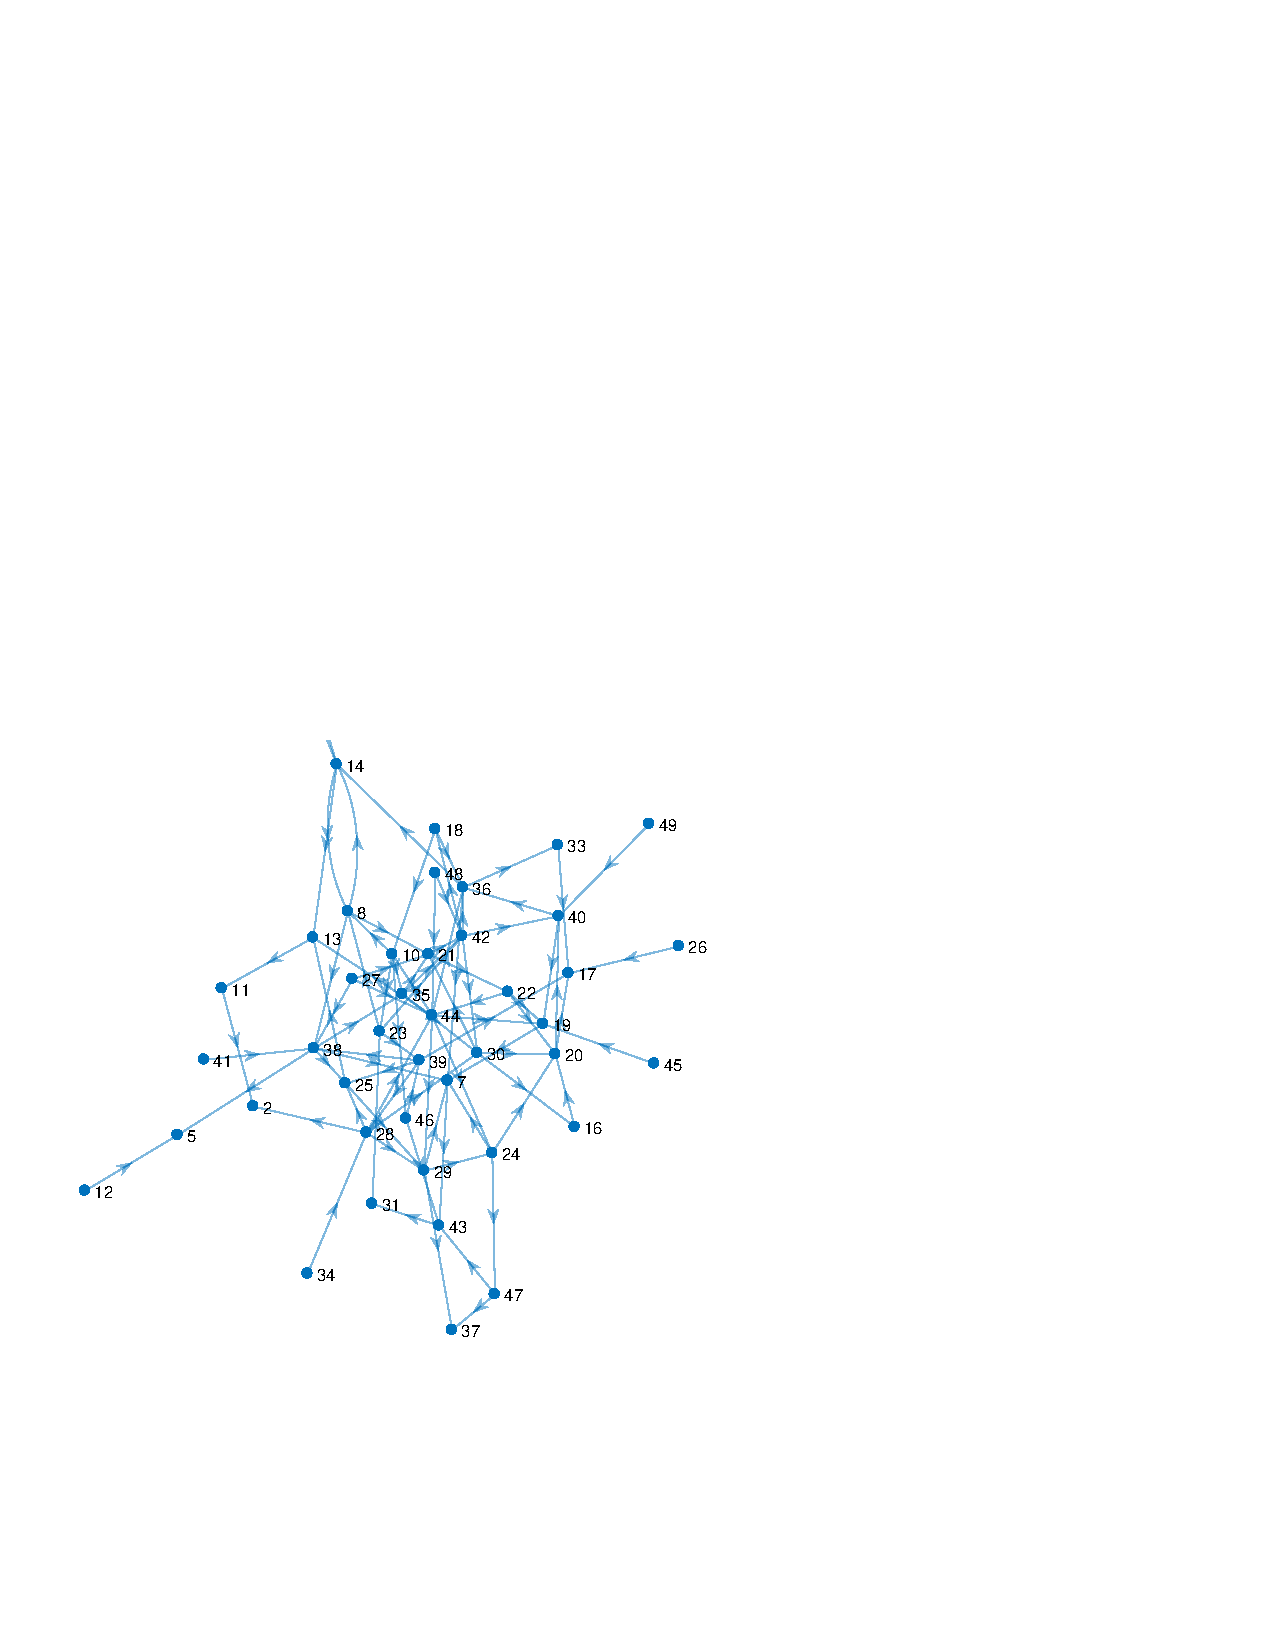
\includegraphics[width=0.8\linewidth]{dag}
%\caption{A Directed Acyclic Graph of the Running AUTOSAR Software Application, Runnables = 50, Paths = 35, Activation Patterns shown in Table \ref{tbl_requirements}.}
%\label{fig_application}
%\end{figure}
%\begin{center}
%\small
%\begin{minipage}{.5\textwidth}%
%\centering
%\begin{tabular}{@{}p{0.25cm}lll@{}}
%\toprule
%C& $r_i$ & $(e_{r_im_1}, e_{r_im_2}, e_{r_im_3})$ & $period$\\ \midrule
%\multirow{4}{4em}{c1} 
%&$r_1$ & (0.030, 0.060, 0.090) & 1\\
%&$r_2$ & (0.041, 0.081, 0.122) & 2\\
%&$r_3$ & (0.083, 0.167, 0.250)  & 5\\ 
%&$r_4$ & (0.310, 0.620, 0.930) & 10 \\[0.3em]
%\hline
%\multirow{2}{4em}{c2} 
%&$r_1$ & (0.310, 0.620, 0.930) & 10\\
%&$r_2$ & (0.310, 0.620, 0.930) & 10\\
%&$r_3$ & (0.310, 0.620, 0.930)  & 10\\ 
%&$r_4$ & (0.310, 0.620, 0.930) & 10 \\[0.3em]
%\hline
%\multirow{2}{4em}{c3} 
%&$r_1$ & (0.310, 0.620, 0.930) & 10\\
%&$r_2$ & (0.291, 0.583, 0.874)) & 10\\
%&$r_3$ & (0.291, 0.583, 0.874)  & 20\\ 
%&$r_4$ & (0.291, 0.583, 0.874) & 20 \\[0.3em]
%\hline
%\multirow{2}{4em}{c4} 
%&$r_1$ & (0.291, 0.583, 0.874) & 20\\
%&$r_2$ & (0.291, 0.583, 0.874)) & 10\\
%&$r_3$ & (0.291, 0.583, 0.874)  & 20\\ 
%&$r_4$ & (0.093, 0.186, 0.279) & 50 \\[0.3em]
%\hline
%\multirow{2}{4em}{c5} 
%&$r_1$ & (0.420, 0.841, 1.261) & 100\\
%&$r_2$ & (0.420, 0.841, 1.261)) & 100\\
%&$r_3$ & (0.420, 0.841, 1.261)  & 100\\ 
%&$r_4$ & (0.420, 0.841, 1.261) & 100 \\[0.3em]
%\bottomrule
%\end{tabular}
%\captionof{table}{Specification of Components.}
%\label{tbl_comps_config}
%\end{minipage}~
%\begin{minipage}{.45\textwidth}
%\begin{center}
%    \begin{tabular}{@{}lll@{}}
%    \toprule
%    Activation, $AP$ & Share & Time, ms \\ \midrule
%    $\tau_1$ & 50  & 50\\
%    $\tau_1\rightarrow\tau_2$ & 20  & 100\\
%    $\tau_1\rightarrow\tau_2\rightarrow\tau_3$ & 20  & 200\\
%    $\tau_1\rightarrow\tau_2\rightarrow\tau_3\rightarrow\tau_4$ & 10  & 400\\
%    \bottomrule
%    \end{tabular}
%    \captionof{table}{Activation Patters of Cause-effect Chains, their Share and End-to-end Timing Requirements.}
%    \label{tbl_requirements}
%\end{center}
%\begin{center}
%    \begin{tabular}{@{}llll@{}}
%    \toprule
%    M  & $P_{idle}$& $P_{busy}$& $\lambda$ \\ \midrule
%    $m_1$ & 50.0& 140.0 &1.0E-3  \\
%    $m_2$ & 10.0& 100.0 &1.0E-4  \\
%    $m_3$ & 10.0& 140.0 &1 .0E-5 \\ \bottomrule
%    \end{tabular}
%    \captionof{table}{Computation Nodes Specification.}
%    \label{tbl_nodes_specification}
%\end{center}
%\end{minipage}
%\end{center}

In the next section, we discuss our proposed method to address the considered optimization problem. 
